\documentclass[a4paper,12pt]{article}
\usepackage{graphicx}
\usepackage{amsmath}
\usepackage{hyperref}
\usepackage{geometry}
\usepackage{float}
\usepackage{subcaption}
\geometry{a4paper, margin=0.7in}

\title{
    
\includegraphics[width=3cm]{images/iitblogo.png} \\ % Add your institute's logo
    \vspace{1cm}
    \LARGE \textbf{Oral Squamous Cell Carcinoma}\\
    \vspace{0.2cm}
    \Large A comprehensive proteomics and metabolomics analysis utilizing machine learning algorithms to identify robust molecular classifiers for the early detection of oral squamous cell carcinoma\\
    \vspace{0.5cm}
    \Large \textbf{Project Report: DH 307}\\
    \vspace{0.5cm}
    \Large Soumitra Darshan Nayak \\ 22B0984 \\
    \Large Guide: Prof Sanjeeva Srivastava\\
    \Large Guide: Avinash Singh\\
    \vspace{0.5cm}
    \normalsize \today
}

% \title{Oral Squamous Cell Carcinoma\\Biomarker Identification using Machine Learning Models\\ Project Report}
% \author{Soumitra Darshan Nayak}
% \date{\today}
\date{} % Remove the default date
\begin{document}

\maketitle
\newpage
\begin{abstract}
	This report outlines the work undertaken during the Oral Squamous Cell Carcinoma (OSCC) Research and Development (R\&D) project, focusing on the identification of potential biomarkers for OSCC using proteomics and metabolomics data. OSCC is a prevalent and aggressive form of cancer with low survival rates due to late-stage diagnosis, underscoring the critical need for reliable biomarkers to enable early detection and targeted treatment strategies.

	The study employed a systematic pipeline that began with extensive data preprocessing to handle missing values, normalize datasets, and ensure consistency. This was followed by robust feature selection processes to reduce the high-dimensional data and retain only the most relevant features. Statistical methods such as Orthogonal Partial Least Squares Discriminant Analysis (OPLS-DA) and Partial Least Squares Discriminant Analysis (PLS-DA) were utilized to identify the relevant features from datasets, after which machine learning models were applied to refine the selection and validate the identified biomarkers.

	Key machine learning methods included Logistic Regression with Elastic Net regularization, Random Forest, and Support Vector Machines (SVM) with Recursive Feature Elimination (RFE) \& Lasso Regression. Each model was evaluated using cross-validation techniques to ensure the reliability and generalizability of the results. Furthermore, a comparative analysis of the selected features was performed to identify common proteins and metabolites that could serve as robust biomarkers for OSCC.

	The integration of proteomics and metabolomics data, along with machine learning, enabled the identification of the most discriminative biomarkers, which can potentially enhance early diagnosis, improve prognosis, and guide personalized treatment strategies for OSCC. The findings underscore the importance of combining high-dimensional biological data with advanced computational methods to unravel insights into complex diseases like OSCC, paving the way for improved clinical outcomes.
\end{abstract}

\newpage
\tableofcontents
\newpage
\section{Oral Squamous Cell Carcinoma (OSCC)}
Oral Squamous Cell Carcinoma (OSCC) is one of the most common malignancies of the head and neck, representing a significant global health burden. It typically arises from the epithelial cells of the oral cavity and can spread to other parts of the body if not detected and treated early. Despite advancements in surgical techniques and therapies, the overall survival rate for OSCC remains low due to late-stage diagnosis, often when the disease has already progressed to an advanced stage.

\subsection{Importance of Early Detection and Biomarkers}
Early detection of OSCC is critical for improving patient prognosis, as it significantly increases the chances of successful treatment and recovery. Traditional diagnostic methods, such as physical examination and biopsy, often detect the disease at later stages, where treatment options are limited. Therefore, identifying reliable biomarkers for OSCC is essential to enable early diagnosis, allowing for more effective interventions and personalized treatments.

Biomarkers, such as specific proteins, metabolites, or genetic changes, can serve as valuable indicators for the presence of OSCC at its earliest stages. Through advanced techniques like metabolomics and proteomics, we can identify and validate these biomarkers, facilitating the development of non-invasive diagnostic tests that can detect OSCC in its asymptomatic phase. This approach holds the potential to revolutionize early detection, making it possible to initiate treatment before the disease spreads, thereby improving survival rates and quality of life for patients. In this project, our goal is to identify potential biomarkers, including proteins and metabolites, that can accurately assess the status of a patient, enabling early diagnosis and personalized treatment strategies.
\section{Proteomics Analysis}
\subsection{Introduction}
In the first part of the project, we analyze biomarker proteins for classifying Tumor versus Normal Adjacent Tissue using various machine-learning models.\\
\textbf{Dataset:-} The dataset comprises protein expression data from 84 samples collected from 42 patients (Tumor and Normal from each patient), encompassing 3611 proteins. We applied several models, including Logistic Regression with Elastic Net, Support Vector Machine (SVM) with Recursive Feature Elimination (RFE) \& Lasso Regression, Random Forest, K-Nearest Neighbors (KNN), and Naive Bayes, to identify significant biomarkers.

\subsection{Methodology}
\subsubsection{Using MetaboAnalyst for Feature Reduction}
We utilized MetaboAnalyst 6.0 (\href{https://dev.metaboanalyst.ca/ModuleView.xhtml}{Visit MetaboAnalyst Module View})  to remove unnecessary features from our dataset. The Partial Least Squares Discriminant Analysis (PLS-DA) method was employed, resulting in eight components. Each component provided Variable Importance in Projection (VIP) scores for each protein. We selected only those proteins with \(avg\_vip\_score > 1\), leading to the identification of 894 significant proteins. After that, we reduced our original dataset to retain information on only these top \textbf{894} proteins. The formula for the VIP score is:-

\[
	\text{VIP} = \frac{1}{n}\sum_{i=1}^{n}\left(\frac{\text{Var}(x_i|y)}{\text{Var}(x_i)}\right) \cdot \text{Corr}(x_i,y)^2
\]

where \( n \) is the number of components, \( x_i \) represents the individual proteins, \( \text{Var}(x_i|y) \) is the variance of protein \( x_i \) conditioned on class \( y \), and \( \text{Corr}(x_i,y) \) is the correlation between protein \( x_i \) and the class variable \( y \).

Now, our objective is to identify the optimal subset of these 894 relevant features that contribute most effectively to the classification task.
\begin{figure}[h]
	\centering
	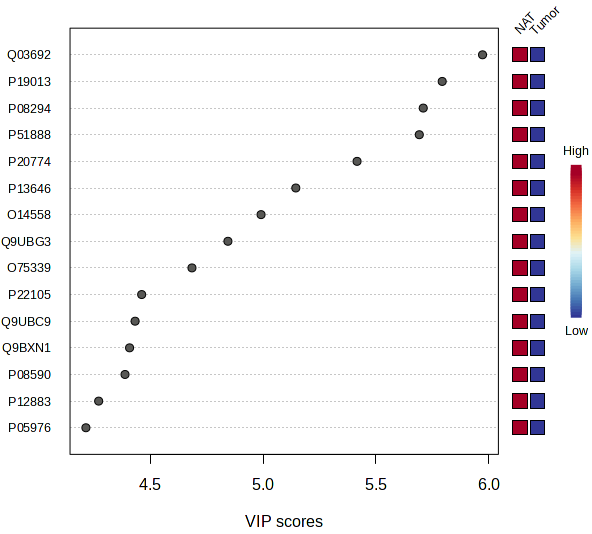
\includegraphics[width=0.6\textwidth]{images/pls_imp_0_dpi72.png}
	\caption{VIP scores of top proteins from MetaboAnalyst 6.0}
	\label{fig:example}
\end{figure}
\subsubsection{Logistic Regression with Elastic Net Regularization}
Logistic regression is a widely used statistical model for binary classification. The Elastic Net regularization combines L1 and L2 penalties, balancing the trade-off between feature selection and multicollinearity. The objective function for Elastic Net is given by:

\[
	L(\beta) = -\sum_{i=1}^{n} \left( y_i \log(p_i) + (1 - y_i) \log(1 - p_i) \right) + \lambda \left( \alpha \|\beta\|_1 + \frac{(1-\alpha)}{2} \|\beta\|_2^2 \right)
\]

where \( p_i \) is the predicted probability, \( \lambda \) is the regularization parameter, and \( \alpha \) controls the mixing of L1 and L2 penalties.\\\\
\textbf{L1 Regularization (Lasso):-}
L1 regularization promotes sparsity in the model by driving some coefficients to exactly zero, thus performing implicit feature selection. This is particularly advantageous when dealing with high-dimensional data, such as in our case, where many features may be irrelevant. By keeping only the most relevant predictors, L1 regularization simplifies the model and enhances interpretability. However, it may also lead to instability in coefficient estimates, especially when features are highly correlated.\\\\
\textbf{L2 Regularization (Ridge):}
In contrast, L2 regularization shrinks the coefficients towards zero without completely eliminating any features. This approach can stabilize the model in the presence of multicollinearity, where predictors are correlated with each other. By applying a penalty proportional to the square of the coefficient values, L2 regularization helps maintain all features while reducing their influence on the model predictions.

Elastic Net regularization combines both L1 (Lasso) and L2 (Ridge) penalties, allowing us to achieve a balance between their individual strengths.
We selected the top 50 features from this model using the \texttt{SelectFromModel} method using the feature relevance.
\subsubsection{Support Vector Machine (SVM) with L1 Regularization}
SVM is a powerful classification technique that finds the optimal hyperplane to separate classes in the feature space. In our implementation, we used a linear kernel with L1 regularization. The decision boundary is determined by:

\[
	w^T x + b = 0
\]

where \( w \) is the weight vector, \( x \) is the input vector, and \( b \) is the bias. The top 27 features with non-zero coefficients were selected from the fitted model using the `SelectFromModel' approach.

We also tried a Support Vector Machine (SVM) model with Recursive Feature Elimination (RFE) for feature selection. RFE iteratively removes the least important features, identifying significant predictors for our classification task. The SVM with RFE achieved an accuracy of approximately 100\% using 5-fold cross-validation.

While RFE effectively selects features, it may lead to overfitting. To address this, we applied L1 regularization, which not only performs feature selection but also penalizes large coefficients. This approach mitigates overfitting, particularly in high-dimensional spaces, by shrinking some coefficients to zero, thus simplifying the model and enhancing its generalizability. By retaining only the most relevant features, we reduce the complexity associated with irrelevant predictors.


\subsubsection{Random Forest}
Random Forest is an ensemble learning method that constructs multiple decision trees during training and outputs the mode of the classes for classification tasks. It is robust to overfitting and works well for high-dimensional data. The feature importance is calculated as:

\[
	\text{Importance}(f) = \sum_{t=1}^{T} \frac{N_{t}}{N} \cdot \Delta Gini_t
\]

where \( N_t \) is the number of samples in tree \( t \) and \( \Delta Gini_t \) is the decrease in Gini impurity contributed by feature \( f \). We selected the top 50 features based on importance scores to retrain the model and got a 5-fold cross-validation accuracy of around 97\%.


\subsubsection{K-Nearest Neighbors (KNN) and Naive Bayes}
Both KNN and Naive Bayes classifiers were tested using the top common selected features. KNN classifies a data point based on the majority class among its \( k \) nearest neighbours, while Naive Bayes applies Bayes' theorem with the assumption of independence among features:

\[
	P(y|X) = \frac{P(X|y)P(y)}{P(X)}
\]
We found around 94\% accuracy with both KNN and Naive Bayes using only the top 5 common features from the selected features of the above models.
\subsection{Results of Different Models}
\subsubsection{Logistic Regression with Elastic Net regularisation}
The Logistic Regression model, utilizing Elastic Net regularization, successfully identified the top 50 proteins from the dataset. After selecting the top features, we reduced the train and test datasets to only contain these top 50 proteins and then retrained the logistic regression model with this modified dataset. The accuracy achieved by the Logistic Regression model was 94\% on the reduced test set and mean cross-validation accuracy (train set): 0.84.

\begin{figure}[H]
	\centering
	% Confusion Matrix
	\begin{minipage}[b]{0.45\textwidth}
		\centering
		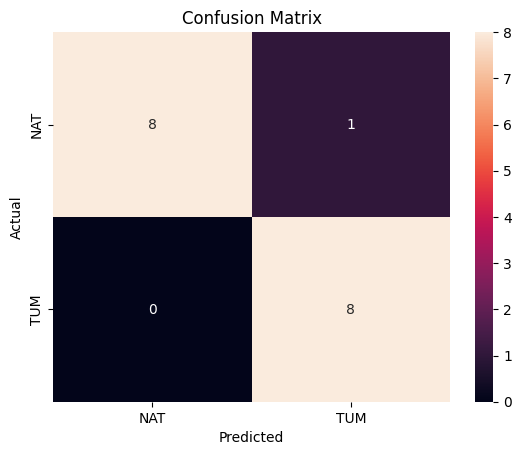
\includegraphics[width=\textwidth]{images/lc.png}
		\caption{Confusion Matrix of logistic regression model}
		\label{fig:confusion_matrix_logreg}
	\end{minipage}
	\hfill
	\begin{minipage}[b]{0.45\textwidth}
		\centering
		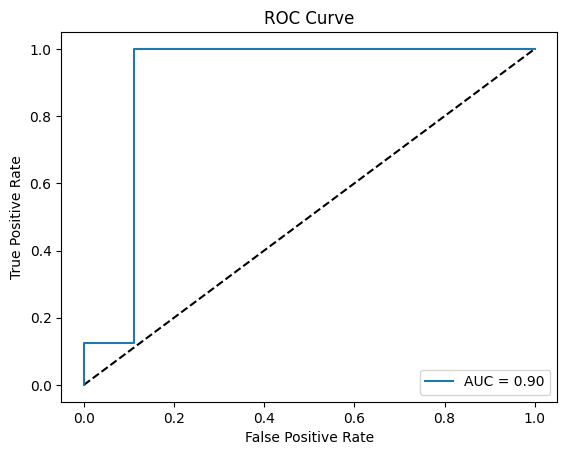
\includegraphics[width=\textwidth]{images/lr.png}
		\caption{Roc curve of logistic regression model}
		\label{fig:roc_curve_logreg}
	\end{minipage}
\end{figure}
The top 50 proteins identified by the model as per their UniProt IDs, are as follows:
\begin{itemize}
	\item \texttt{Q96IU4}, \texttt{P30838}, \texttt{Q9BXN1}, \texttt{P55957}, \texttt{P35613}, \texttt{Q13895}, \texttt{O75339}, \texttt{P23946}, \texttt{Q03692}, \texttt{Q05707}
	\item \texttt{P02461}, \texttt{Q8NBJ5}, \texttt{P15088}, \texttt{P52943}, \texttt{Q9UBG3}, \texttt{O75718}, \texttt{Q53TN4}, \texttt{O95865}, \texttt{P07099}, \texttt{P34913}
	\item \texttt{Q96AY3}, \texttt{O95302}, \texttt{P29992}, \texttt{P22352}, \texttt{P07305}, \texttt{P00738}, \texttt{Q92598}, \texttt{P13646}, \texttt{P19013}, \texttt{Q13751}
	\item \texttt{Q9UHB6}, \texttt{Q08AI8}, \texttt{P27338}, \texttt{Q99685}, \texttt{Q99735}, \texttt{P35749}, \texttt{O43795}, \texttt{Q8TCD5}, \texttt{P20774}, \texttt{Q6UWY5}
	\item \texttt{P02763}, \texttt{P13674}, \texttt{Q08174}, \texttt{P51888}, \texttt{Q13308}, \texttt{P50454}, \texttt{Q9NR46}, \texttt{P08195}, \texttt{P08294}, \texttt{P02786}
\end{itemize}


\subsubsection{Random Forest Model}
The Random Forest model identified the top 50 proteins from the dataset. After selecting the top features, we reduced the train and test datasets to only contain these top 50 proteins and retrained the Random Forest model with the modified dataset. The accuracy achieved by the Random Forest model was 94\% on the reduced test set and mean cross-validation accuracy (train set): 0.97.

\begin{figure}[H]
	\centering
	% Confusion Matrix
	\begin{minipage}[b]{0.45\textwidth}
		\centering
		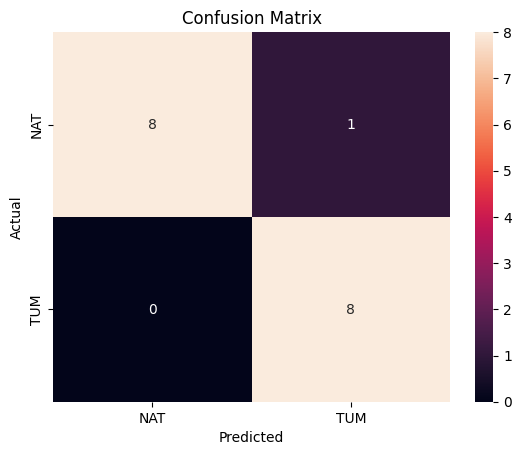
\includegraphics[width=\textwidth]{images/rc.png}
		\caption{Confusion Matrix of Random Forest model}
		\label{fig:confusion_matrix_rf}
	\end{minipage}
	\hfill
	% ROC Curve
	\begin{minipage}[b]{0.45\textwidth}
		\centering
		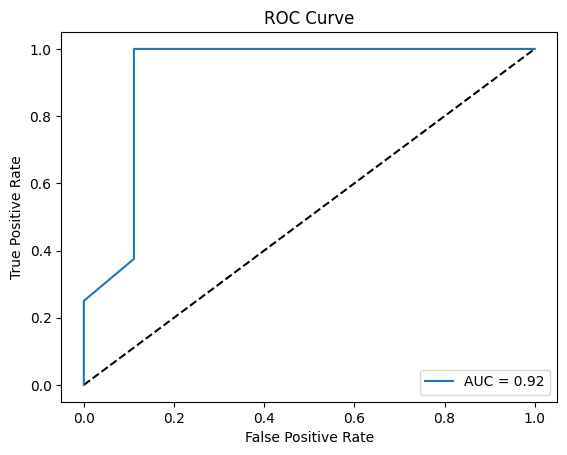
\includegraphics[width=\textwidth]{images/rr.png}
		\caption{ROC Curve of Random Forest model}
		\label{fig:roc_rf}
	\end{minipage}
\end{figure}

The top 50 proteins identified by the Random Forest model, according to their UniProt IDs, are as follows:
\begin{itemize}
	\item \texttt{P27338}, \texttt{Q13813}, \texttt{O43795}, \texttt{P08195}, \texttt{O95865}, \texttt{Q6UWY5}, \texttt{Q99735}, \texttt{P08294}, \texttt{Q9UN36}, \texttt{Q8N335}
	\item \texttt{Q16853}, \texttt{P00746}, \texttt{P29992}, \texttt{Q03692}, \texttt{P05166}, \texttt{Q13228}, \texttt{Q53TN4}, \texttt{Q08J23}, \texttt{Q92598}, \texttt{O95302}
	\item \texttt{P30086}, \texttt{P55268}, \texttt{P51888}, \texttt{Q9Y6K5}, \texttt{P20774}, \texttt{Q9UEY8}, \texttt{Q07507}, \texttt{O14933}, \texttt{Q96AG4}, \texttt{Q16762}
	\item \texttt{Q13509}, \texttt{P05091}, \texttt{P13674}, \texttt{Q13308}, \texttt{O00339}, \texttt{P49189}, \texttt{P00167}, \texttt{Q9HBL0}, \texttt{P17812}, \texttt{Q9H0A0}
	\item \texttt{Q969V3}, \texttt{P24821}, \texttt{Q92506}, \texttt{P51608}, \texttt{Q9BX66}, \texttt{P25311}, \texttt{P32455}, \texttt{P51884}, \texttt{P14927}, \texttt{Q63ZY3}
\end{itemize}


\subsubsection{Support Vector Machine (SVM) Model}
The Support Vector Machine (SVM) model, employing Lasso regularization, selected the top 27 proteins from the dataset. After selecting these proteins, we reduced the train and test datasets to only include these features and retrained the SVM model. The SVM model achieved an accuracy of 94\% on the reduced test set and mean cross-validation accuracy (train set): 0.98.

The top 27 proteins identified by the SVM model, according to their UniProt IDs, are as follows:
\begin{itemize}
	\item \texttt{P55957}, \texttt{O75339}, \texttt{Q03692}, \texttt{Q9NZJ6}, \texttt{P52943}, \texttt{Q03001}, \texttt{P34913}, \texttt{Q96AY3}, \texttt{P35269}
	\item \texttt{P00738}, \texttt{Q92598}, \texttt{Q92743}, \texttt{P01876}, \texttt{P13646}, \texttt{Q2M2I5}, \texttt{Q9NX58}, \texttt{P27338}, \texttt{Q9Y623}
	\item \texttt{Q8TCD5}, \texttt{Q6UWY5}, \texttt{P02763}, \texttt{Q08174}, \texttt{Q15063}, \texttt{P51888}, \texttt{Q9BXM0}, \texttt{Q9UBD6}, \texttt{Q66K66}
\end{itemize}
\begin{figure}[H]
	\centering
	% Confusion Matrix
	\begin{minipage}[b]{0.45\textwidth}
		\centering
		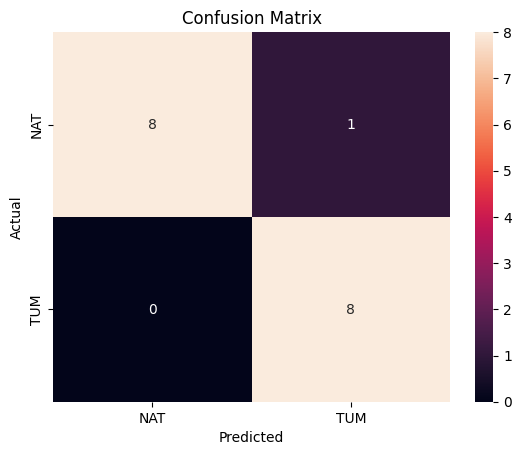
\includegraphics[width=\textwidth]{images/slc.png}
		\caption{Confusion Matrix of SVM model}
		\label{fig:confusion_matrix_svm}
	\end{minipage}
	\hfill
	% ROC Curve
	\begin{minipage}[b]{0.45\textwidth}
		\centering
		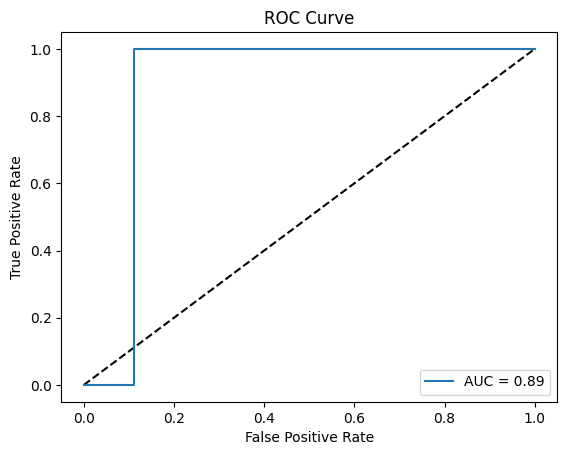
\includegraphics[width=\textwidth]{images/slr.png}
		\caption{ROC Curve of SVM model}
		\label{fig:roc_svm}
	\end{minipage}
\end{figure}



\subsubsection{Comparison of Common Proteins Across Models}
After comparing the proteins selected by all three models, we identified 5 common proteins that appeared in the feature sets of all models. These proteins, with their corresponding UniProt IDs, are:
\begin{itemize}
	\item \texttt{P27338}
	\item \texttt{P51888}
	\item \texttt{Q03692}
	\item \texttt{Q6UWY5}
	\item \texttt{Q92598}
\end{itemize}

To evaluate the significance of these proteins, we modified the dataset to include only these five proteins. Upon retraining the models using only these features, we achieved an accuracy of 94\% with the Random Forest model and 88\% with both the Logistic Regression and SVM models. So, the Random Forest Model emerged as the best-performing model among those evaluated.

\begin{figure}[h]
	\centering
	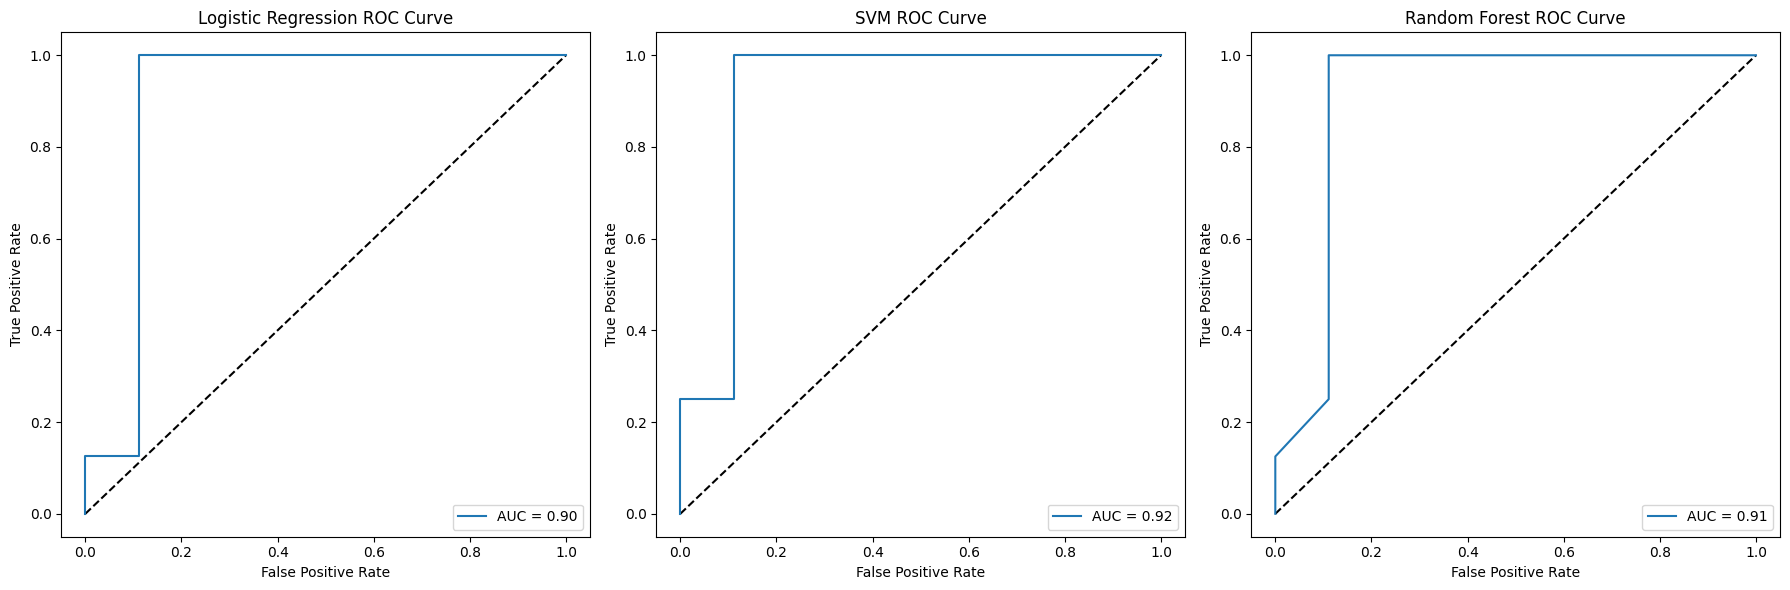
\includegraphics[width=1\textwidth]{images/top5_combined.png}
	\caption{ROC Curves for Common Proteins Across Models}
	\label{fig:top5_combined}
\end{figure}
\subsubsection{Observational Trends}
We plotted the boxplots for the 5 common proteins, along with their corresponding t-statistics and p-values, using data from the original dataset of 42 patients. The boxplots highlight a decreasing trend for the first four proteins from NAT to Tumor and an increasing trend for the last protein from NAT to Tumor. Below are the boxplots for these 5 common proteins:

\begin{figure}[H]
	\centering
	% First Row
	\begin{minipage}[b]{0.32\textwidth}
		\centering
		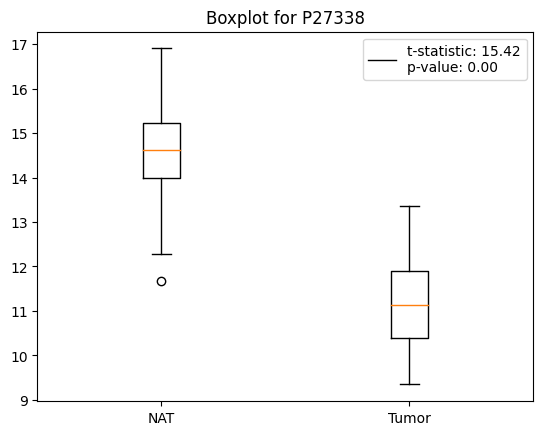
\includegraphics[width=\textwidth]{images/1.png}
		\caption{Boxplot for P27338}
		\label{fig:boxplot_Q03692}
	\end{minipage}
	\hfill
	\begin{minipage}[b]{0.32\textwidth}
		\centering
		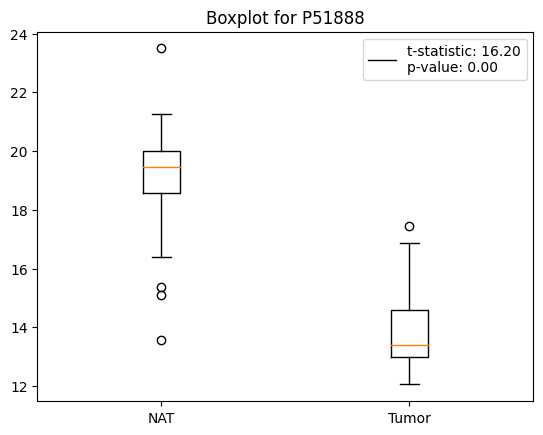
\includegraphics[width=\textwidth]{images/2.png}
		\caption{Boxplot for P51888}

		\label{fig:boxplot_Q6UWY5}
	\end{minipage}
	\hfill
	\begin{minipage}[b]{0.32\textwidth}
		\centering
		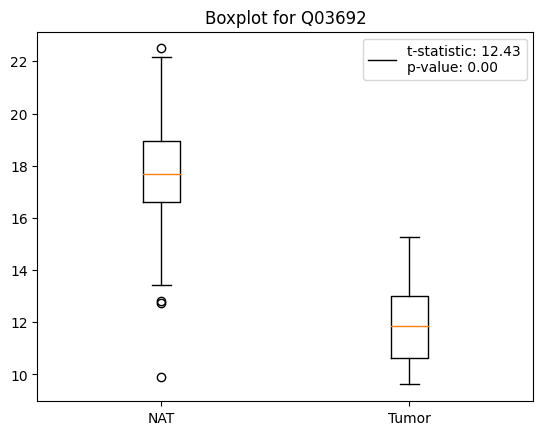
\includegraphics[width=\textwidth]{images/3.png}
		\caption{Boxplot for Q03692}

		\label{fig:boxplot_Q92598}
	\end{minipage}

	% Second Row
	\vspace{1em}
	\begin{minipage}[b]{0.4\textwidth}
		\centering
		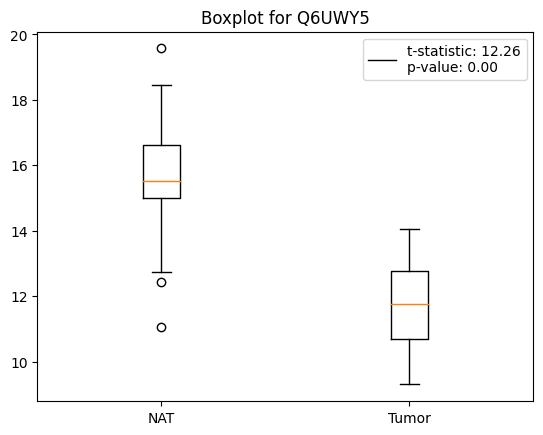
\includegraphics[width=\textwidth]{images/4.png}
		\caption{Boxplot for Q6UWY5}

	\end{minipage}
	\hfill
	\begin{minipage}[b]{0.4\textwidth}
		\centering
		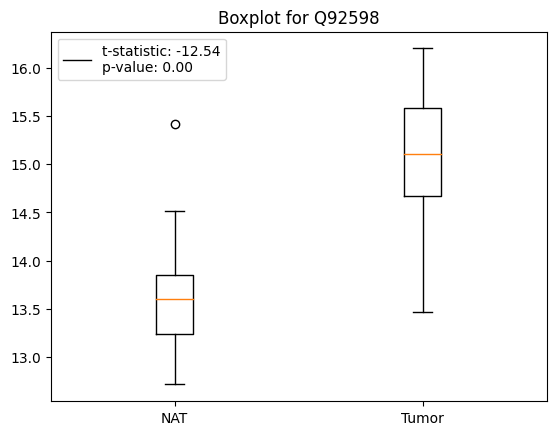
\includegraphics[width=\textwidth]{images/5.png}
		\caption{Boxplot for Q92598}

		\label{fig:boxplot_P51888}
	\end{minipage}
\end{figure}





\subsection{Validation of Selected Biomarkers}

\textbf{CPTAC} (Clinical Proteomic Tumor Analysis Consortium) is a collaborative initiative by the National Cancer Institute (NCI) aimed at advancing the understanding of cancer biology through the comprehensive characterization of tumour proteomes. By analyzing cancer samples from various tumour types, CPTAC seeks to identify molecular biomarkers for early detection, diagnosis, and treatment.

To validate the selected biomarkers, we utilized the \texttt{CPTAC\_TumorVsNormal.xlsx} dataset, which comprises approximately 172 tumour and normal samples, each characterized by 9,666 distinct genes. We employed KNN imputation with a neighbourhood of 5 to address any missing values in the dataset. Next, we mapped our top-selected proteins to their corresponding genes and filtered the genes to retain only those that represent our top features. We evaluated the performance of the Random Forest (RF), Support Vector Machine (SVM), and Logistic Regression models, achieving 5-fold cross-validation accuracies of 97.5\%, 97.85\%, and 95.83\%, respectively, along with 100\% accuracy on the test set for the SVM model and around 96\% for both RF and Logistic Regression. The SVM model exhibited the best performance, followed closely by the RF model on the CPTAC dataset.


% \subsection{Results}
% After applying the models, we identified several common features across the different algorithms. The intersection of the selected features across the models resulted in 5 common features, demonstrating their significance in classifying tumour versus normal cells. The top 5 common features yielded a 5-fold cross-validation accuracy of approximately 97.8\% on the CPTAC dataset using the SVM model, indicating strong predictive power.

% \subsection{Conclusion}
% The analysis demonstrates the efficacy of various machine-learning models in identifying critical biomarker proteins. Future research could focus on validating these findings with larger datasets and investigating alternative algorithms to improve accuracy. Additionally, it will be essential to assess the biological significance of the selected top biomarkers to ensure their reliability.

\section{Metabolomics Analysis}
\subsection{Introduction}
In the second part of the project, we have focused on the metabolomics study. While proteomics data provides insight into protein-level changes, metabolomics data highlights alterations in metabolic pathways. This study focuses on the analysis of two metabolomics datasets:
\begin{itemize}
	\item \textbf{3Groups-OSCC\_PM\_Normal.xlsx}: Contains 41 columns representing mixed groups (OSCC, PM, Normal) with 1,378 metabolites per column across two sheets (Positive and Negative).
	\item \textbf{TumorVsNAT\_Metabolomics\_Tissue.xlsx}: Contains 31 columns (mixed Tumor and NAT groups) with 3,771 metabolites per column across two sheets (Positive and Negative).
\end{itemize}
We integrate these metabolomics analyses with the previously conducted proteomics study to identify the top discriminative features using statistical and machine learning techniques.

\subsection{Methodology}

\subsubsection{Data Preprocessing}
\begin{itemize}
	\item Each dataset was preprocessed to ensure consistent handling of missing values, normalization, and scaling.
	\item Metabolomics data was analyzed separately for each dataset's Positive and Negative sheets.

\end{itemize}

\subsubsection{MetaboAnalyst Analysis}
\begin{itemize}
	\item For the \textbf{Tumor vs NAT} dataset:
	      \begin{itemize}
		      \item Orthogonal Partial Least Squares Discriminant Analysis (OPLS-DA) was performed in MetaboAnalyst 6.0.
		      \item Features with predictive variance score greater than a certain threshold were selected, narrowing the list to approximately top 500 metabolites.
	      \end{itemize}
	\item For the \textbf{3Groups} dataset:
	      \begin{itemize}
		      \item Partial Least Squares Discriminant Analysis (PLS-DA) was applied using MetaboAnalyst 6.0.
		      \item The average score across 8 components was calculated, and a threshold was applied to select approximately top 250 metabolites.
	      \end{itemize}
\end{itemize}

After this we have reduced our dataset to contain only these top metabolites, which would be further refined using different machine learning models. Below are the graphs of the vip scores of the top metabolites selected by the MetaboAnalyst 6.0.
\begin{figure}[H]
	\centering
	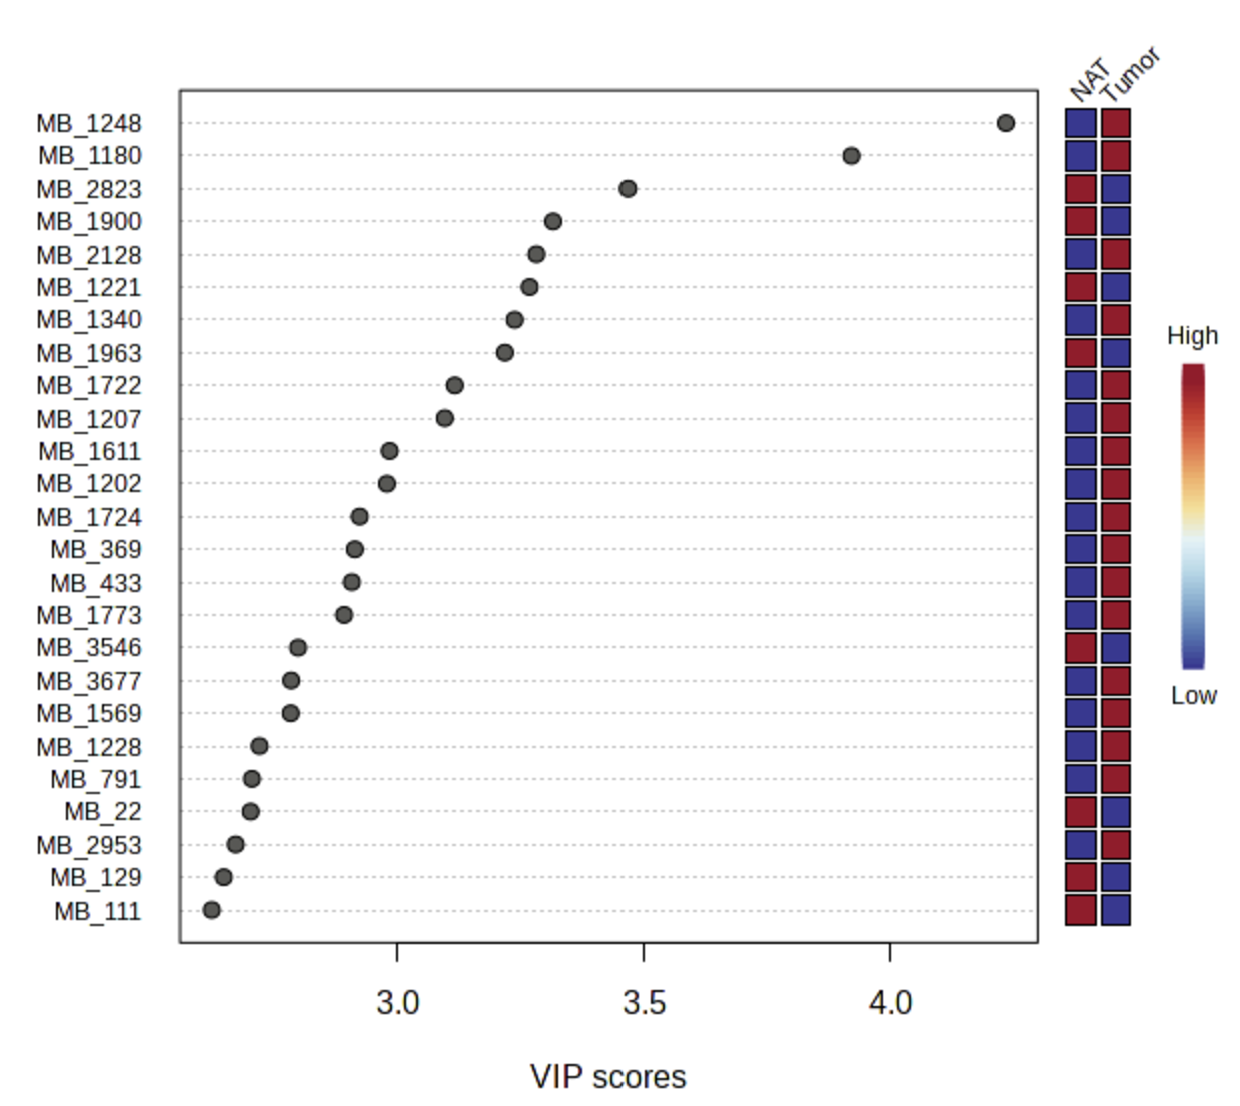
\includegraphics[width=0.7\textwidth]{images/oplsda_positive.png}
	\caption{VIP scores of top metabolites (Positive sheet - Tum vs NAT)}
	\label{fig:vip_positive_tum_nat}
\end{figure}

\begin{figure}[H]
	\centering
	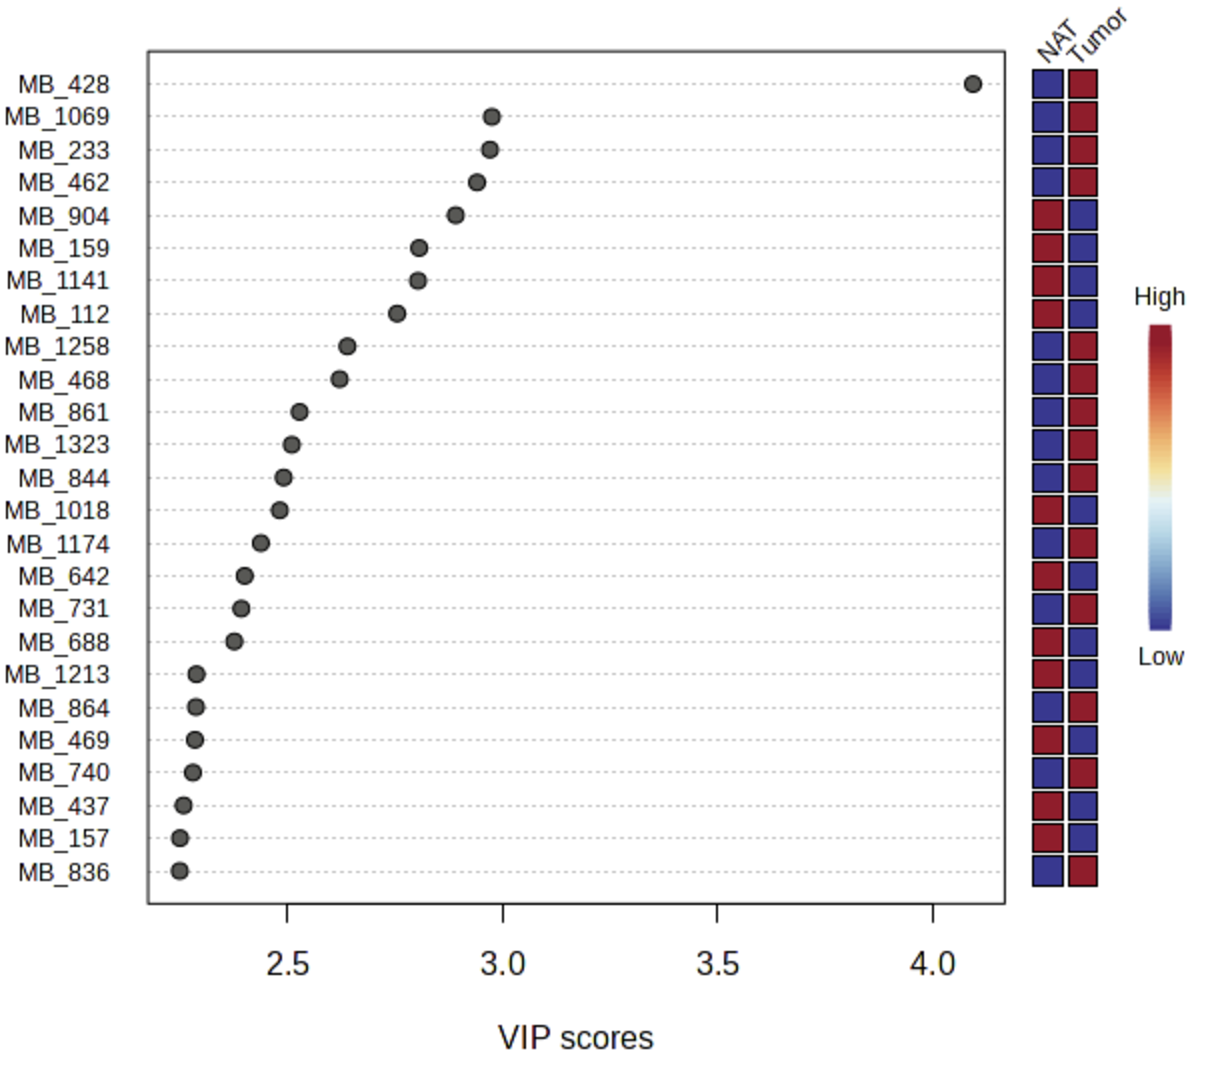
\includegraphics[width=0.7\textwidth]{images/oplsda_negative.png}
	\caption{VIP scores of top metabolites (Negative sheet - Tum vs NAT)}
	\label{fig:vip_negative_tum_nat}
\end{figure}

\begin{figure}[H]
	\centering
	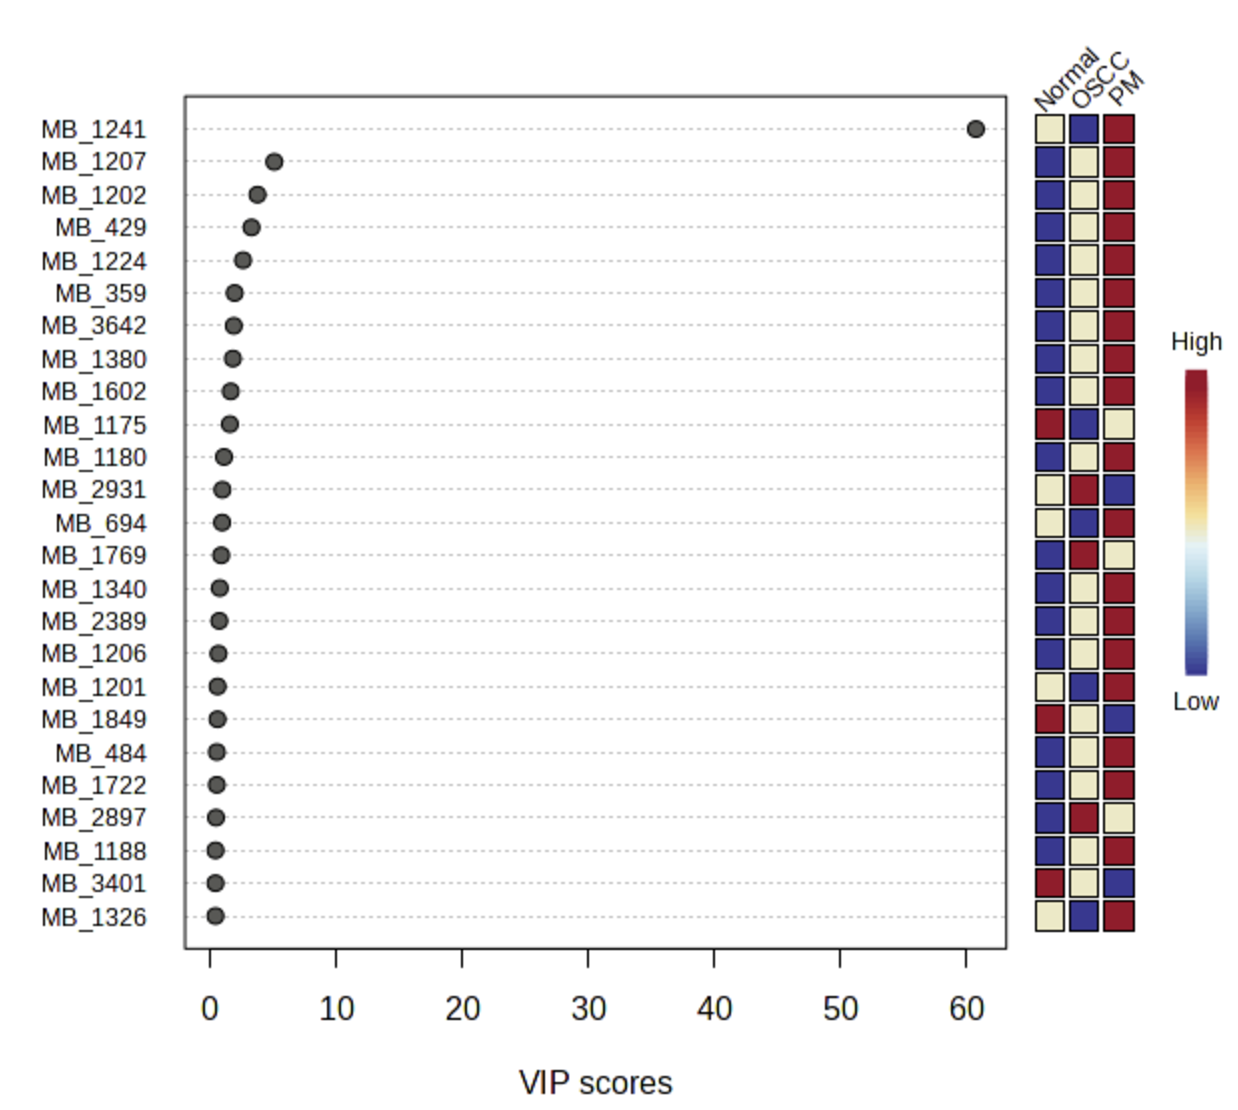
\includegraphics[width=0.6\textwidth]{images/3group_positive.png}
	\caption{VIP scores of top metabolites (Positive sheet - 3Groups: OSCC, PM, Normal)}
	\label{fig:vip_positive_3groups}
\end{figure}

\begin{figure}[H]
	\centering
	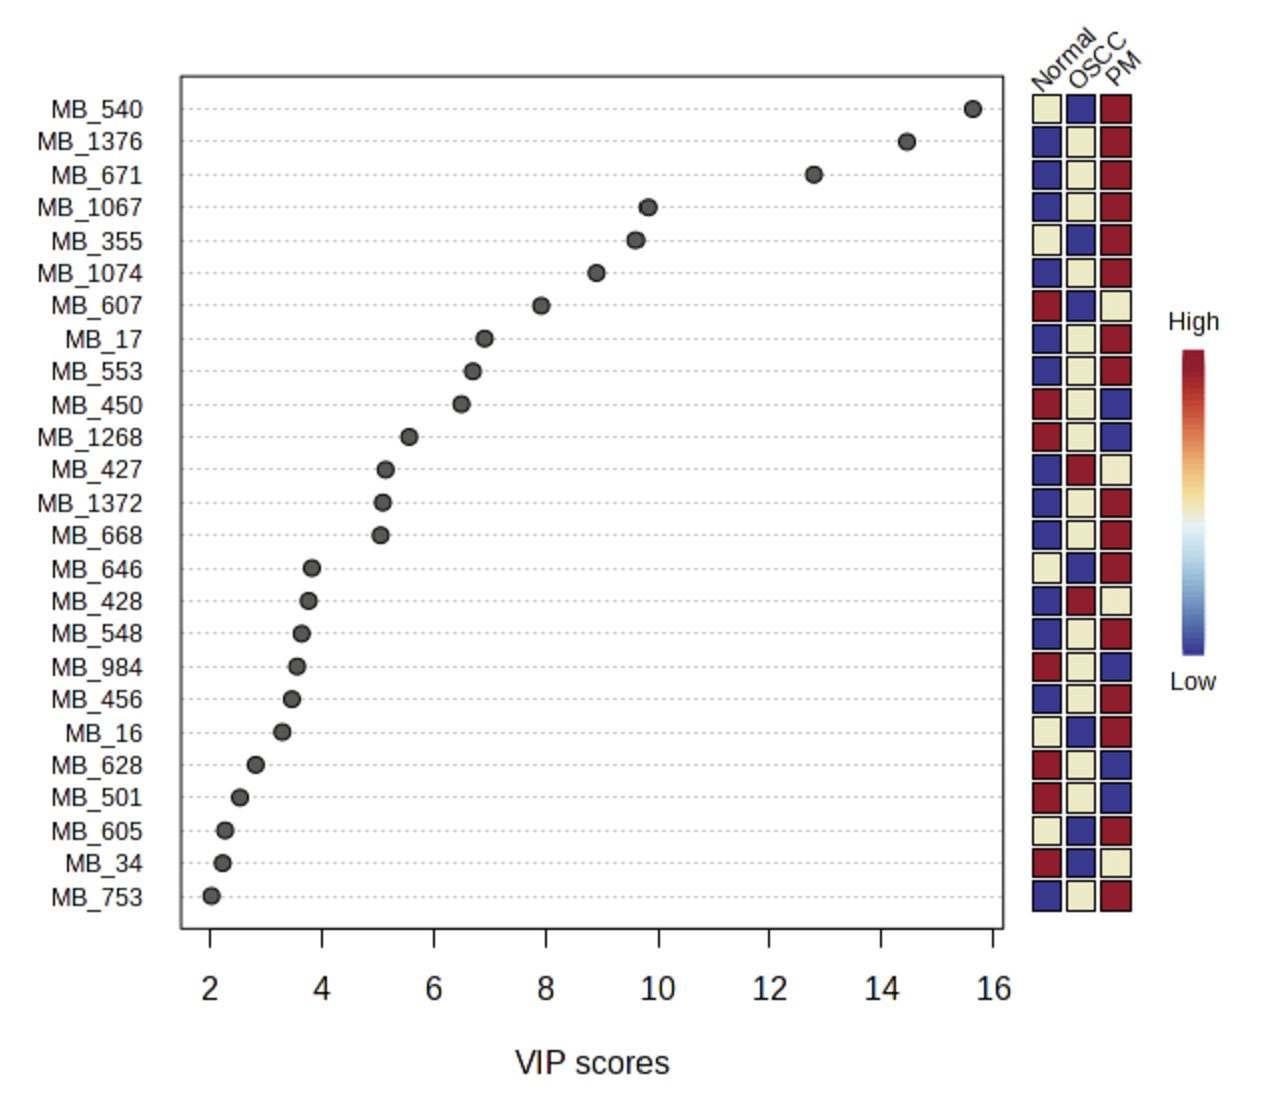
\includegraphics[width=0.6\textwidth]{images/3group_negative.png}
	\caption{VIP scores of top metabolites (Negative sheet - 3Groups: OSCC, PM, Normal)}
	\label{fig:vip_negative_3groups}
\end{figure}

\subsubsection{Machine Learning Models}
To further refine the features, the following machine learning models were employed:
\begin{enumerate}
	\item \textbf{Logistic Regression with Elastic Net Regularization}:\\
	      The logistic regression model was implemented with Elastic Net regularization, which combines L1 (Lasso) and L2 (Ridge) penalties to balance feature selection and regularization. The model parameters were tuned using 5-fold cross-validation, ensuring robust performance evaluation. We have selected top 25 features using the \texttt{SelectFromModel} method.
	\item \textbf{Random Forest}:\\
	      A Random Forest classifier was implemented, and hyperparameters were optimized using \texttt{GridSearchCV} with 5-fold cross-validation. The tuned parameters included: \textbf{Number of Trees} (100, 200, 500), \textbf{Max Depth} (10, 20, None), and \textbf{Minimum Samples Split} (2, 5, 10). The best hyperparameters were identified and used to train the model. Feature importance scores were extracted, and the top 25 features were selected for further analysis.

	\item \textbf{SVM with L1 Regularization}:\\
	      A Linear Support Vector Machine (SVM) with L1 regularization was implemented to perform simultaneous classification and feature selection. The configuration included: \textbf{Penalty:} \(L1\), enabling sparse feature selection; \textbf{Dual Optimization:} set to \texttt{False} for compatibility with smaller datasets; and \textbf{Maximum Iterations:} increased to 10,000 for convergence. Using L1 regularization, the model selected top features based upon non-zero coefficients.\\
	      \hspace*{2em}To adapt the Linear Support Vector Machine (SVM) model with L1 regularization for multiclass classification, several modifications were made. The dataset labels were binarized using \texttt{label\_binarize} to facilitate the calculation of individual ROC curves for each class. A multiclass confusion matrix was generated to assess classification performance across the categories, namely \textit{Normal}, \textit{PM}, and \textit{OSCC}. Feature selection was performed using non-zero coefficients from the L1-regularized model to select the top 25 features.



\end{enumerate}

\subsection{Results of Different Models}

\subsubsection{Logistic Regression with Elastic Net}
\begin{figure}[H]
	\centering

	% Row 1, Subfigure 1
	\begin{subfigure}[b]{0.45\textwidth}
		\centering
		\begin{subfigure}[b]{0.49\textwidth}
			\centering
			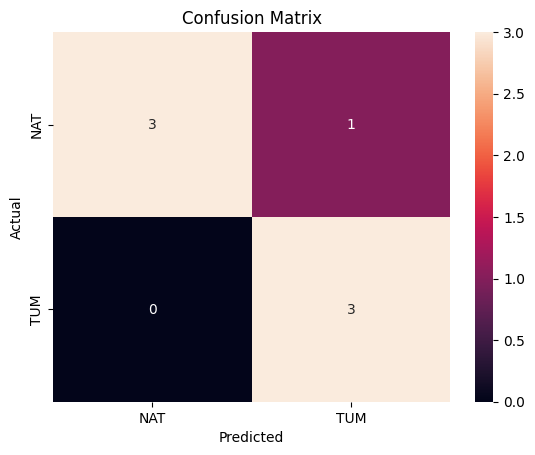
\includegraphics[width=\textwidth]{images/2lpc.png}  % Replace with your image path
			\caption{Confusion Matrix}
			\label{fig:fig1}
		\end{subfigure}
		\hfill
		\begin{subfigure}[b]{0.49\textwidth}
			\centering
			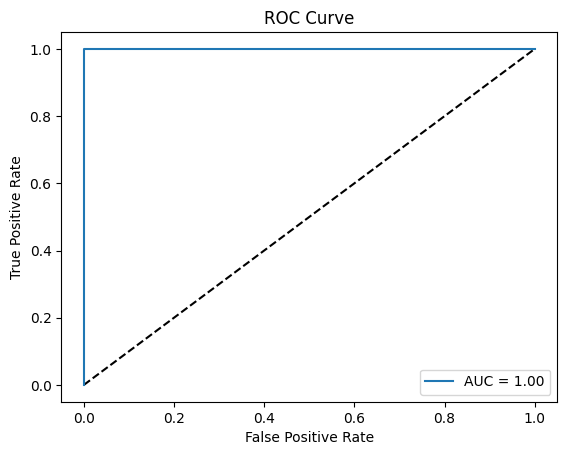
\includegraphics[width=\textwidth]{images/2lpr.png}  % Replace with your image path
			\caption{ROC curve \& AUC}
			\label{fig:fig2}
		\end{subfigure}
		\caption{TUM vs NAT (Positive)}
		\label{subfig:1}
	\end{subfigure}
	\hfill
	% Row 1, Subfigure 2
	\begin{subfigure}[b]{0.45\textwidth}
		\centering
		\begin{subfigure}[b]{0.49\textwidth}
			\centering
			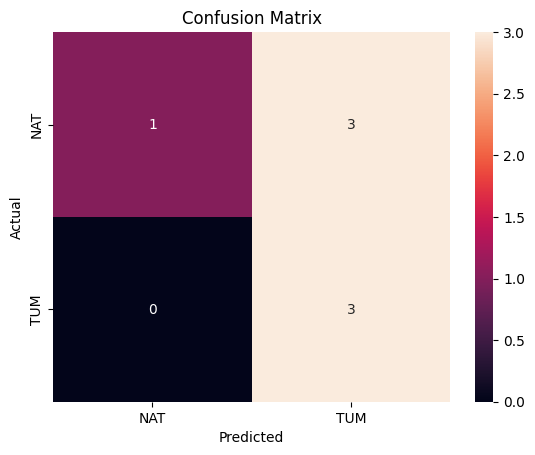
\includegraphics[width=\textwidth]{images/2lnc.png}  % Replace with your image path
			\caption{Confusion Matrix}
			\label{fig:fig3}
		\end{subfigure}
		\hfill
		\begin{subfigure}[b]{0.49\textwidth}
			\centering
			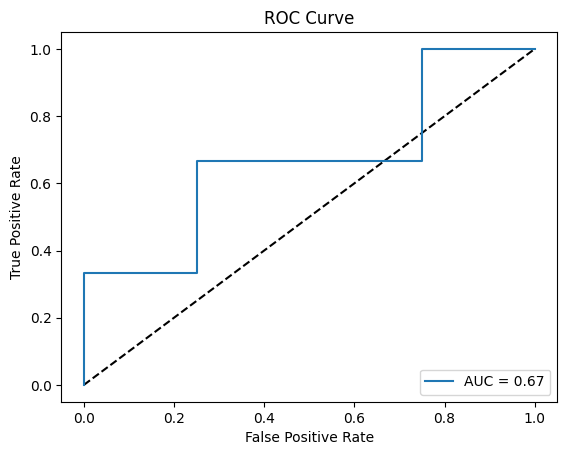
\includegraphics[width=\textwidth]{images/2lnr.png}  % Replace with your image path
			\caption{ROC curve \& AUC}
			\label{fig:fig4}
		\end{subfigure}
		\caption{TUM vs NAT (Negative)}
		\label{subfig:2}
	\end{subfigure}

	% Row 2, Subfigure 3
	\begin{subfigure}[b]{0.45\textwidth}
		\centering
		\begin{subfigure}[b]{0.49\textwidth}
			\centering
			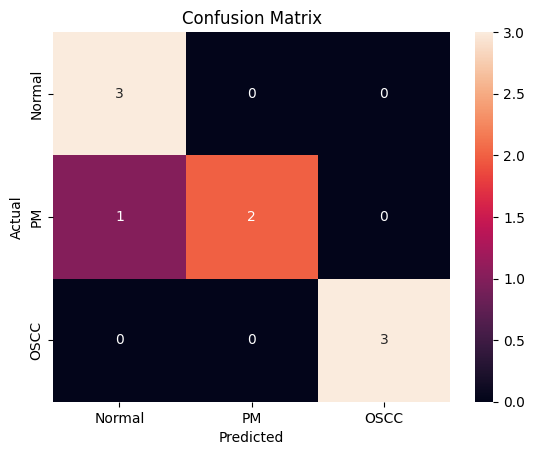
\includegraphics[width=\textwidth]{images/3lpc.png}  % Replace with your image path
			\caption{Confusion Matrix}
			\label{fig:fig5}
		\end{subfigure}
		\hfill
		\begin{subfigure}[b]{0.49\textwidth}
			\centering
			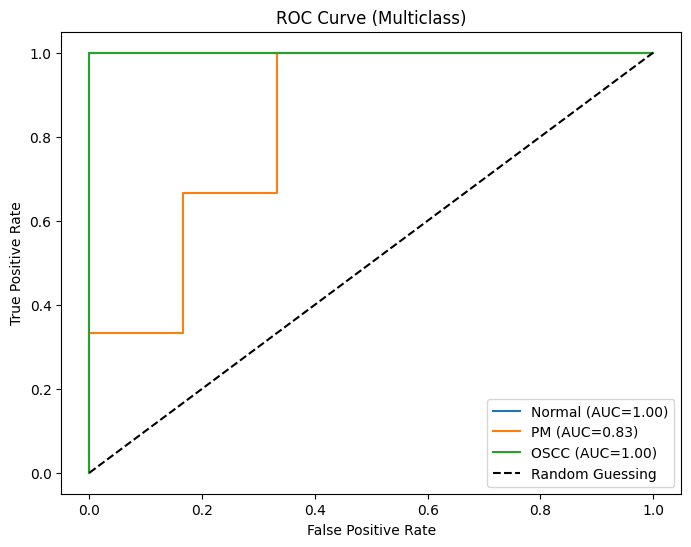
\includegraphics[width=\textwidth]{images/3lpr.png}  % Replace with your image path
			\caption{ROC curve \& AUC}
			\label{fig:fig6}
		\end{subfigure}
		\caption{3groups (Positive)}
		\label{subfig:3}
	\end{subfigure}
	\hfill
	% Row 2, Subfigure 4
	\begin{subfigure}[b]{0.45\textwidth}
		\centering
		\begin{subfigure}[b]{0.49\textwidth}
			\centering
			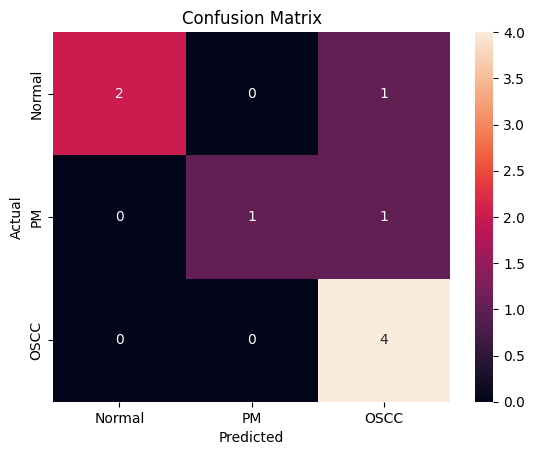
\includegraphics[width=\textwidth]{images/3lnc.png}  % Replace with your image path
			\caption{Confusion Matrix}
			\label{fig:fig7}
		\end{subfigure}
		\hfill
		\begin{subfigure}[b]{0.49\textwidth}
			\centering
			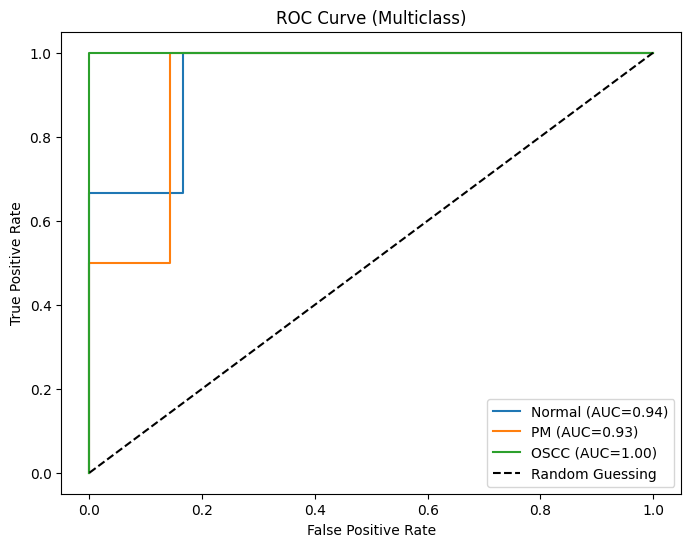
\includegraphics[width=\textwidth]{images/3lnr.png}  % Replace with your image path
			\caption{ROC curve \& AUC}
			\label{fig:fig8}
		\end{subfigure}
		\caption{3groups (Negative)}
		\label{subfig:4}
	\end{subfigure}

	\caption{Model outputs from datasets with top 25 features}
	\label{fig:grid}
\end{figure}
The logistic regression model is not performing well as compared to the other 2 models with accuracy approximately 60\% in each dataset.
\subsubsection{Random Forest Model}
\begin{figure}[H]
	\centering

	% Row 1, Subfigure 1
	\begin{subfigure}[b]{0.45\textwidth}
		\centering
		\begin{subfigure}[b]{0.49\textwidth}
			\centering
			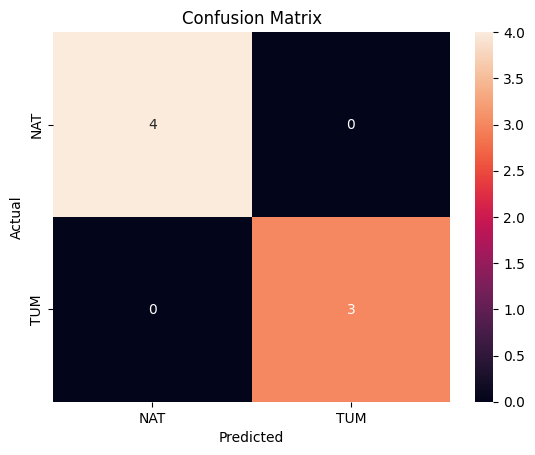
\includegraphics[width=\textwidth]{images/2prc.png}  % Replace with your image path
			\caption{Confusion Matrix}
			\label{fig:fig1}
		\end{subfigure}
		\hfill
		\begin{subfigure}[b]{0.49\textwidth}
			\centering
			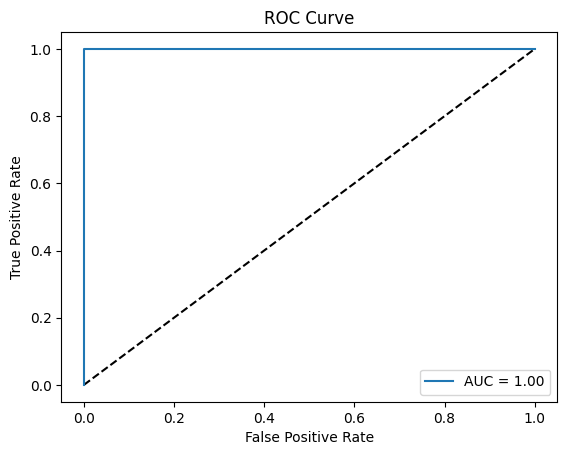
\includegraphics[width=\textwidth]{images/2prr.png}  % Replace with your image path
			\caption{ROC curve \& AUC}
			\label{fig:fig2}
		\end{subfigure}
		\caption{TUM vs NAT (Positive)}
		\label{subfig:1}
	\end{subfigure}
	\hfill
	% Row 1, Subfigure 2
	\begin{subfigure}[b]{0.45\textwidth}
		\centering
		\begin{subfigure}[b]{0.49\textwidth}
			\centering
			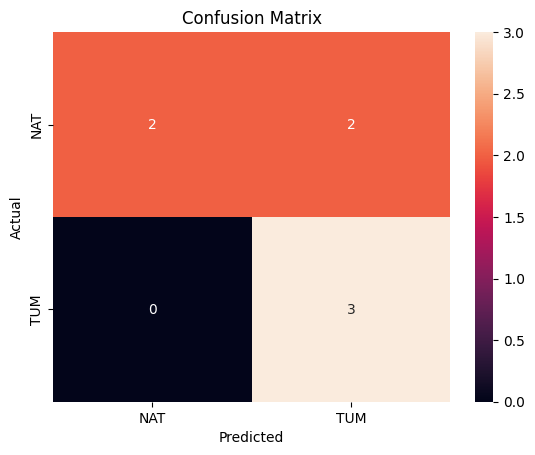
\includegraphics[width=\textwidth]{images/2nrc.png}  % Replace with your image path
			\caption{Confusion Matrix}
			\label{fig:fig3}
		\end{subfigure}
		\hfill
		\begin{subfigure}[b]{0.49\textwidth}
			\centering
			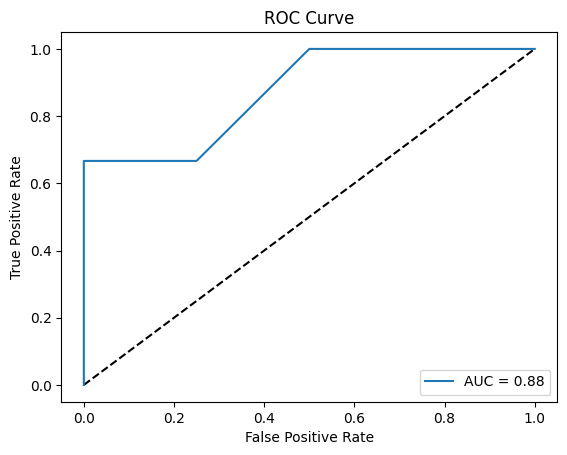
\includegraphics[width=\textwidth]{images/2nrr.png}  % Replace with your image path
			\caption{ROC curve \& AUC}
			\label{fig:fig4}
		\end{subfigure}
		\caption{TUM vs NAT (Negative)}
		\label{subfig:2}
	\end{subfigure}

	% Row 2, Subfigure 3
	\begin{subfigure}[b]{0.45\textwidth}
		\centering
		\begin{subfigure}[b]{0.49\textwidth}
			\centering
			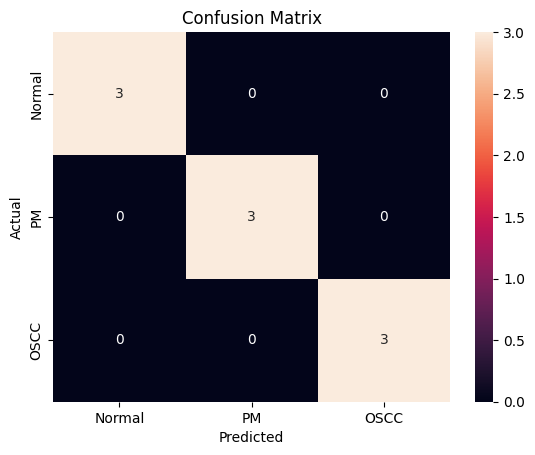
\includegraphics[width=\textwidth]{images/3prc.png}  % Replace with your image path
			\caption{Confusion Matrix}
			\label{fig:fig5}
		\end{subfigure}
		\hfill
		\begin{subfigure}[b]{0.49\textwidth}
			\centering
			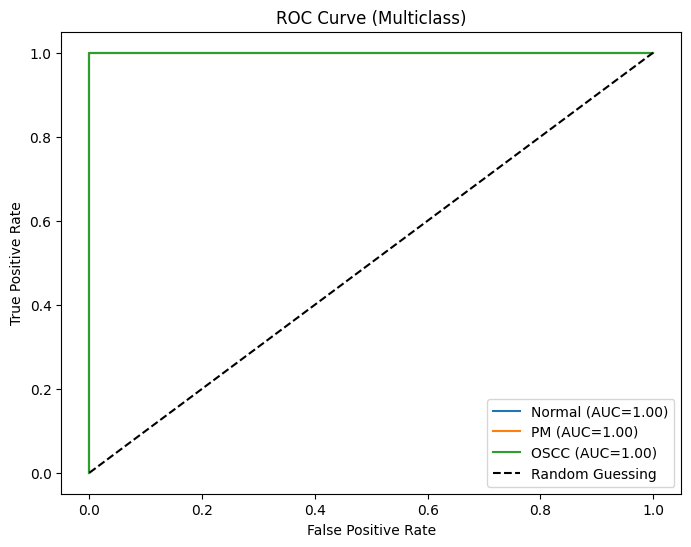
\includegraphics[width=\textwidth]{images/3prr.png}  % Replace with your image path
			\caption{ROC curve \& AUC}
			\label{fig:fig6}
		\end{subfigure}
		\caption{3groups (Positive)}
		\label{subfig:3}
	\end{subfigure}
	\hfill
	% Row 2, Subfigure 4
	\begin{subfigure}[b]{0.45\textwidth}
		\centering
		\begin{subfigure}[b]{0.49\textwidth}
			\centering
			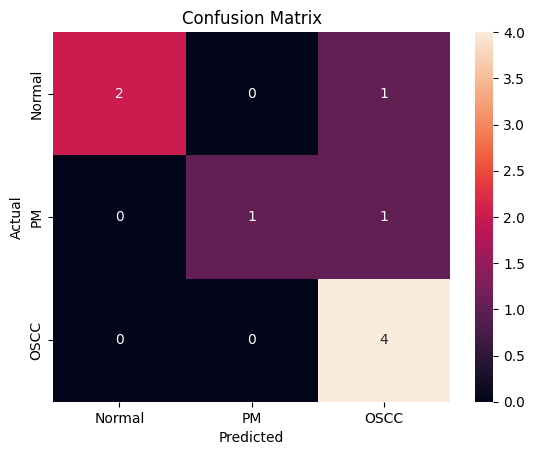
\includegraphics[width=\textwidth]{images/3nrc.png}  % Replace with your image path
			\caption{Confusion Matrix}
			\label{fig:fig7}
		\end{subfigure}
		\hfill
		\begin{subfigure}[b]{0.49\textwidth}
			\centering
			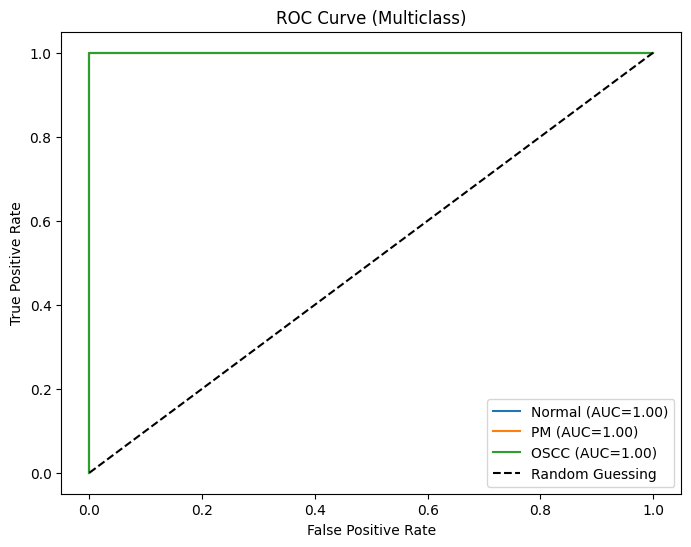
\includegraphics[width=\textwidth]{images/3nrr.png}  % Replace with your image path
			\caption{ROC curve \& AUC}
			\label{fig:fig8}
		\end{subfigure}
		\caption{3groups (Negative)}
		\label{subfig:4}
	\end{subfigure}

	\caption{Model outputs from datasets with top 25 features}
	\label{fig:grid}
\end{figure}
The Random Forest model is outperforming the other two models in positive datasets with accuracy on the test sets 100\% in each positive dataset.
\subsubsection{SVM with L1 regularisation}
\begin{figure}[H]
	\centering

	% Row 1, Subfigure 1
	\begin{subfigure}[b]{0.45\textwidth}
		\centering
		\begin{subfigure}[b]{0.49\textwidth}
			\centering
			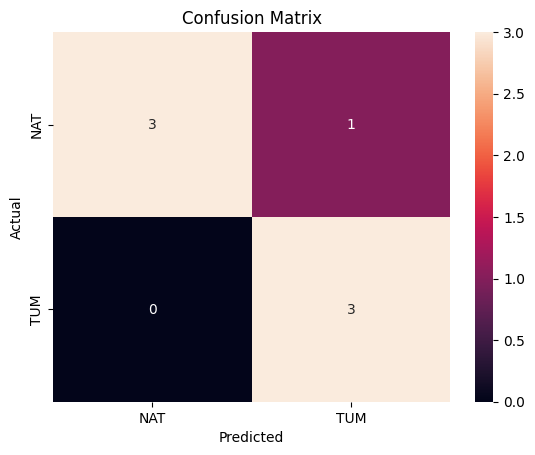
\includegraphics[width=\textwidth]{images/2psl1c.png}  % Replace with your image path
			\caption{Confusion Matrix}
			\label{fig:fig1}
		\end{subfigure}
		\hfill
		\begin{subfigure}[b]{0.49\textwidth}
			\centering
			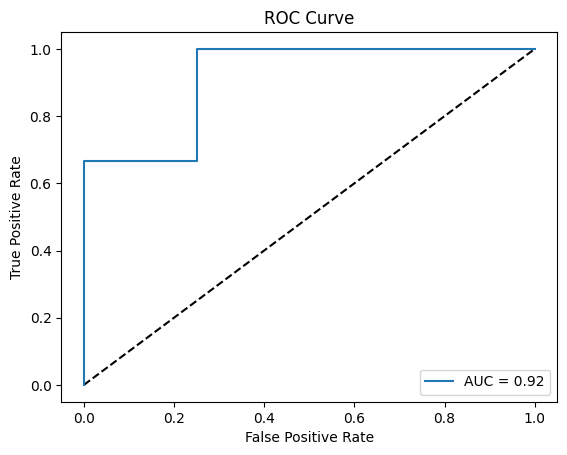
\includegraphics[width=\textwidth]{images/2psl1r.png}  % Replace with your image path
			\caption{ROC curve \& AUC}
			\label{fig:fig2}
		\end{subfigure}
		\caption{TUM vs NAT (Positive)}
		\label{subfig:1}
	\end{subfigure}
	\hfill
	% Row 1, Subfigure 2
	\begin{subfigure}[b]{0.45\textwidth}
		\centering
		\begin{subfigure}[b]{0.49\textwidth}
			\centering
			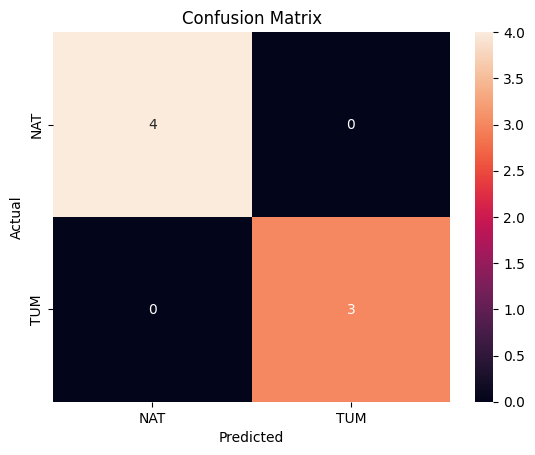
\includegraphics[width=\textwidth]{images/2nsl1c.png}  % Replace with your image path
			\caption{Confusion Matrix}
			\label{fig:fig3}
		\end{subfigure}
		\hfill
		\begin{subfigure}[b]{0.49\textwidth}
			\centering
			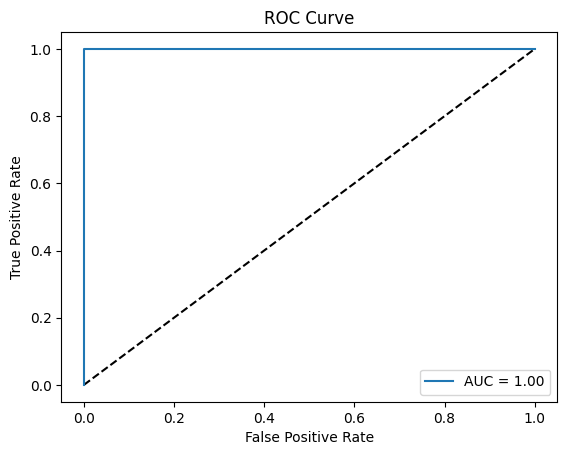
\includegraphics[width=\textwidth]{images/2nsl1r.png}  % Replace with your image path
			\caption{ROC curve \& AUC}
			\label{fig:fig4}
		\end{subfigure}
		\caption{TUM vs NAT (Negative)}
		\label{subfig:2}
	\end{subfigure}

	% Row 2, Subfigure 3
	\begin{subfigure}[b]{0.45\textwidth}
		\centering
		\begin{subfigure}[b]{0.49\textwidth}
			\centering
			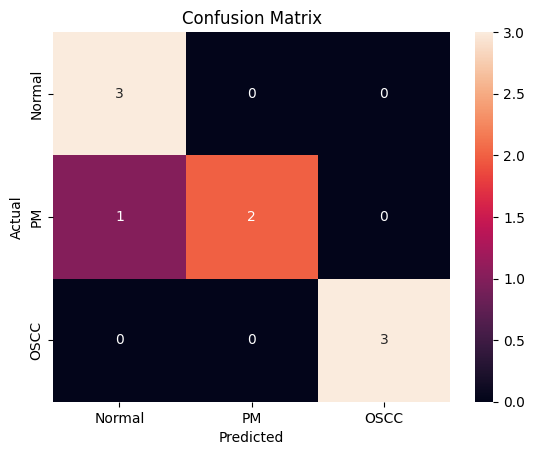
\includegraphics[width=\textwidth]{images/3psl1c.png}  % Replace with your image path
			\caption{Confusion Matrix}
			\label{fig:fig5}
		\end{subfigure}
		\hfill
		\begin{subfigure}[b]{0.49\textwidth}
			\centering
			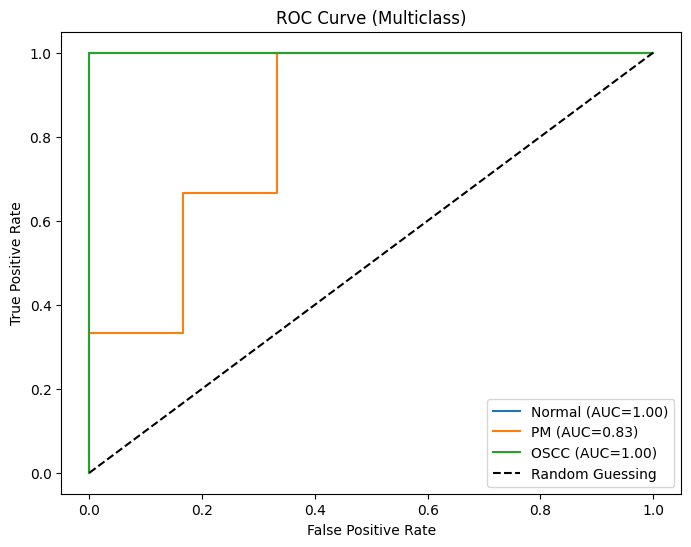
\includegraphics[width=\textwidth]{images/3psl1r.png}  % Replace with your image path
			\caption{ROC curve \& AUC}
			\label{fig:fig6}
		\end{subfigure}
		\caption{3groups (Positive)}
		\label{subfig:3}
	\end{subfigure}
	\hfill
	% Row 2, Subfigure 4
	\begin{subfigure}[b]{0.45\textwidth}
		\centering
		\begin{subfigure}[b]{0.49\textwidth}
			\centering
			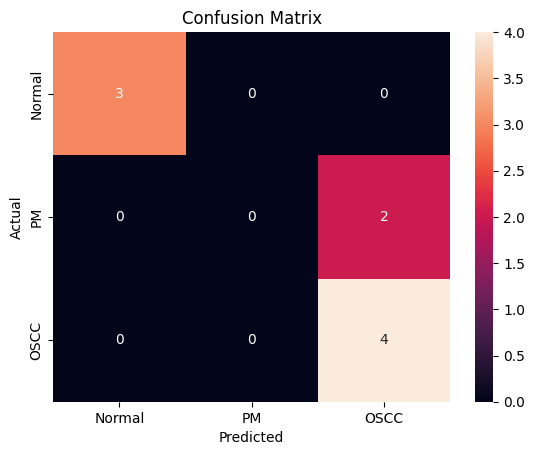
\includegraphics[width=\textwidth]{images/3nsl1c.png}  % Replace with your image path
			\caption{Confusion Matrix}
			\label{fig:fig7}
		\end{subfigure}
		\hfill
		\begin{subfigure}[b]{0.49\textwidth}
			\centering
			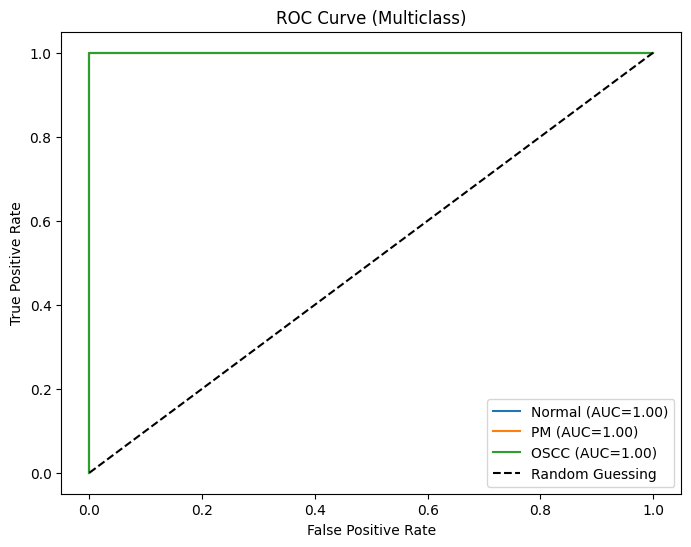
\includegraphics[width=\textwidth]{images/3nsl1r.png}  % Replace with your image path
			\caption{ROC curve \& AUC}
			\label{fig:fig8}
		\end{subfigure}
		\caption{3groups (Negative)}
		\label{subfig:4}
	\end{subfigure}

	\caption{Model outputs from datasets with top 25 features}
	\label{fig:grid}
\end{figure}
The SVM model with L1 regularisation is outperfoming the other two models in the negative datasets with accuracy of 100\% in the Tum Vs Nat (negative) dataset and around 80\% in the 3groups (negative) dataset.
The confusion matrices provide insights into the classification accuracy, while the ROC curves highlight the model's ability to distinguish between classes across datasets. We can see from the above plots that the Random Forest model consistently performs better than the SVM with L1 regularisation across different datasets.\\
I have put the top 25 features selected by various models from all the 4 datasets in the result section of the metabolomics directory (\href{run:./metabolomics/results}{Results Directory}). I could not find any top feature which is common in the top 25 selected features by the Random Forest model across 4 datasets.

\section{Conclusion}
This study demonstrated the power of integrating proteomics and metabolomics datasets with advanced machine learning techniques to identify robust biomarkers for the early detection of Oral Squamous Cell Carcinoma (OSCC). By leveraging high-dimensional datasets, we applied systematic feature selection and classification methodologies, achieving promising results in both the proteomics and metabolomics domains.

\subsection*{Key Findings}
\begin{enumerate}
	\item \textbf{Proteomics Analysis}:
	      \begin{itemize}
		      \item Using machine learning models such as Logistic Regression with Elastic Net, Support Vector Machines (SVM) with L1 regularization, and Random Forest, we identified a subset of highly relevant proteins from a dataset of 3,611 proteins.
		      \item Notably, five proteins (P27338, P51888, Q03692, Q6UWY5, Q92598) were common across all models, demonstrating their potential as robust biomarkers for OSCC classification.
	      \end{itemize}
	\item \textbf{Metabolomics Analysis}:
	      \begin{itemize}
		      \item A combination of statistical techniques (e.g., OPLS-DA and PLS-DA) and machine learning models narrowed down thousands of metabolites to a concise set of top features.
		      \item Models such as Random Forest and SVM demonstrated superior performance, achieving accuracies up to 100\% on specific datasets, highlighting the discriminative power of the selected metabolites.
	      \end{itemize}
	\item \textbf{Model Comparison}:
	      \begin{itemize}
		      \item The Random Forest model emerged as the most consistent performer across various datasets, particularly excelling in positive metabolomics datasets, achieving 100\% accuracy on test sets.
		      \item The SVM model with L1 regularization was particularly effective in negative datasets, demonstrating its adaptability for different dataset characteristics.
	      \end{itemize}
\end{enumerate}

\subsection*{Significance}
By integrating the top 25 features from metabolomics with proteomics biomarkers, we developed a comprehensive biomarker panel. This integrative approach has the potential to significantly improve the early detection of OSCC, enabling personalized treatment strategies and better patient outcomes. The ability to identify common biomarkers across independent datasets further strengthens the reliability of these findings.

\subsection*{Limitations and Future Directions}
\begin{enumerate}
	\item \textbf{Validation}:
	      \begin{itemize}
		      \item Although the models achieved high accuracy, further validation on independent datasets, such as those from CPTAC, is necessary to confirm the generalizability of the identified biomarkers.
		      \item External validation using larger, more diverse patient cohorts will enhance the translational potential of these biomarkers.
	      \end{itemize}
	\item \textbf{Clinical Applicability}:
	      \begin{itemize}
		      \item Developing cost-effective, non-invasive diagnostic tools based on the identified biomarkers will be a crucial next step. Techniques like liquid biopsy and targeted metabolomics can be explored for this purpose.
	      \end{itemize}
	\item \textbf{Integration with Clinical Data}:
	      \begin{itemize}
		      \item Incorporating clinical variables, such as patient demographics and medical history, alongside omics data may improve model performance and provide more comprehensive insights into OSCC progression.
	      \end{itemize}
\end{enumerate}

In conclusion, this study highlights the utility of combining machine learning techniques with high-dimensional biological data to uncover critical insights into OSCC. The integration of proteomics and metabolomics features holds significant promise for improving early detection, guiding therapeutic interventions, and ultimately enhancing clinical outcomes. Continued efforts in validation and clinical translation are imperative to realize the full potential of these findings.


\newpage
\begin{thebibliography}{5}

	\bibitem{judith2021}
	Judith, Laura, et al. ``Applications of Machine Learning in Human Microbiome Studies: A Review on Feature Selection, Biomarker Identification, Disease Prediction and Treatment." \textit{Frontiers in Microbiology}, vol. 12, 2021, p. 634511. https://doi.org/10.3389/fmicb.2021.634511. Accessed 1 Oct. 2024.

	\bibitem{shi2020}
	Shi, Zhiao, et al. ``Feature Selection Methods for Protein Biomarker Discovery from Proteomics or Multiomics Data." \textit{Molecular \& Cellular Proteomics}, vol. 20, 2020, p. 100083. https://doi.org/10.1016/j.mcpro.2021.100083. Accessed 1 Oct. 2024.

	\bibitem{leclercq2019}
	Leclercq, Mickael, et al. ``Large-Scale Automatic Feature Selection for Biomarker Discovery in High-Dimensional OMICs Data." \textit{Frontiers in Genetics}, vol. 10, 2019, p. 449967. https://doi.org/10.3389/fgene.2019.00452. Accessed 1 Oct. 2024.

	\bibitem{altashi2023}
	Al-Tashi, Qasem, et al. ``Machine Learning Models for the Identification of Prognostic and Predictive Cancer Biomarkers: A Systematic Review." \textit{International Journal of Molecular Sciences}, vol. 24, no. 9, 2023. https://doi.org/10.3390/ijms24097781. Accessed 1 Oct. 2024.

	\bibitem{altashi2023}
	Chen, Yangzi, et al. ``Metabolomic Machine Learning Predictor for Diagnosis and Prognosis of Gastric Cancer." Nature Communications, vol. 15, no. 1, 2024, pp. 1-13,  https://doi.org/10.1038/s41467-024-46043-y. Accessed 27 Nov. 2024.

	\bibitem{metaboanalyst}
	Chong, J., Wishart, D.S., Xia, J. ``Using MetaboAnalyst 6.0 for Comprehensive and Integrative Metabolomics Data Analysis." Current Protocols in Bioinformatics, vol. 68, 2019, e86. https://dev.metaboanalyst.ca/ModuleView.xhtml. Accessed 1 Oct. 2024.

\end{thebibliography}



\end{document}
